% !TeX program = xelatex
% !TeX program = xelatex

\documentclass[12pt]{article}

\usepackage{lineno,changepage,lipsum}
\usepackage[colorlinks=true,urlcolor=blue]{hyperref}
\usepackage{fontspec}
\usepackage{xeCJK}
\usepackage{tabularx}
\setCJKfamilyfont{chanto}{AozoraMinchoRegular.ttf}
\setCJKfamilyfont{tegaki}{Mushin.otf}
\usepackage[CJK,overlap]{ruby}
\usepackage{hhline}
\usepackage{multirow,array,amssymb}
\usepackage[croatian]{babel}
\usepackage{soul}
\usepackage[usenames, dvipsnames]{color}
\usepackage{wrapfig,booktabs}
\renewcommand{\rubysep}{0.1ex}
\renewcommand{\rubysize}{0.75}
\usepackage[margin=50pt]{geometry}
\modulolinenumbers[2]

\usepackage{pifont}
\newcommand{\cmark}{\ding{51}}%
\newcommand{\xmark}{\ding{55}}%

\definecolor{faded}{RGB}{100, 100, 100}

\renewcommand{\arraystretch}{1.2}

%\ruby{}{}
%$($\href{URL}{text}$)$

\newcommand{\furigana}[2]{\ruby{#1}{#2}}
\newcommand{\tegaki}[1]{
	\CJKfamily{tegaki}\CJKnospace
	#1
	\CJKfamily{chanto}\CJKnospace
}

\newcommand{\dai}[1]{
	\vspace{20pt}
	\large
	\noindent\textbf{#1}
	\normalsize
	\vspace{20pt}
}

\newcommand{\fukudai}[1]{
	\vspace{10pt}
	\noindent\textbf{#1}
	\vspace{10pt}
}

\newenvironment{bunshou}{
	\vspace{10pt}
	\begin{adjustwidth}{1cm}{3cm}
	\begin{linenumbers}
}{
	\end{linenumbers}
	\end{adjustwidth}
}

\newenvironment{reibun}{
	\vspace{10pt}
	\begin{tabular}{l l}
}{
	\end{tabular}
	\vspace{10pt}
}
\newcommand{\rei}[2]{
	#1&\textit{#2}\\
}
\newcommand{\reinagai}[2]{
	\multicolumn{2}{l}{#1}\\
	\multicolumn{2}{l}{\hspace{10pt}\textit{#2}}\\
}

\newenvironment{mondai}[1]{
	\vspace{10pt}
	#1
	
	\begin{enumerate}
		\itemsep-5pt
	}{
	\end{enumerate}
	\vspace{10pt}
}

\newenvironment{hyou}{
	\begin{itemize}
		\itemsep-5pt
	}{
	\end{itemize}
	\vspace{10pt}
}

\date{\today}

\CJKfamily{chanto}\CJKnospace
\author{Tomislav Mamić}

\begin{document}
	\dai{\furigana{原稿用紙}{げんこうようし}の使い方}
	
	\fukudai{Izgled papira}
		
	\begin{wrapfigure}{r}{.25\textwidth}
		\centering
		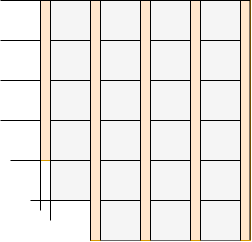
\includegraphics[width=.25\textwidth]{017_pisanje_res/a1.png}
		\caption{izgled papira}
	\end{wrapfigure}

	Na desnoj strani prikazana je rešetka 原稿用紙 papira, preciznije gornji desni kut. Kvadratna polja (マス) u koja se upisuju znakovi složena su u stupce odvojene uskim okomitim prostorom koji služi za upisivanje čitanja težih znakova (ふりがな).
	
	Tradicionalno, papir je položen vodoravno, a tekst se piše okomito prema dolje, s desne strane prema lijevoj. U toj se situaciji ふりがな piše desno od znaka kojem pripada. Moguće ga je koristiti i postavljenog okomito tako da se tekst piše vodoravno s lijeva na desno pa se onda ふりがな nalazi iznad svog znaka. Osim u jednoj iznimnoj situaciji, svaki je znak, uključujući i interpunkciju, smješten u svoje polje.
	
	\fukudai{\furigana{題名}{だいめい}・名前\ - naslov i ime}
	
	\begin{wrapfigure}{r}{.25\textwidth}
		\centering
		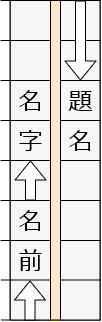
\includegraphics[width=.1\textwidth]{017_pisanje_res/a2.png}
		\caption{naslov i ime}
	\end{wrapfigure}

	Naslov teksta piše se u prvi stupac, tako da se preskoče prva dva ili tri polja. Ako naslov ne stane u prvi stupac, onda je to loš naslov. Ime se piše u sljedeći stupac, tako da se piše prvo (iznad) prezime (名字), a ispod ime (名前). Između imena i prezimena ostavlja se jedno prazno polje, a ime završava jedno polje prije kraja stupca.
	
\end{document}